% biomsample_bib.tex
%
% v1.0 released 12th December 2006 (Dr. S. Sharma, Prof. N. Saxena, and Dr. S. Tahir)
%
% The biomsample.tex file has been amended to highlight
% the proper use of LaTeX2e code with the class file
% and using natbib cross-referencing.
%
\documentclass[useAMS,usenatbib]{biom}
%\documentclass[useAMS,usenatbib,referee]{biom}
%
%
%  Papers submitted to Biometrics should ALWAYS be prepared
%  using the referee option!!!! Clau: does not compile
%
%
% If your system does not have the AMS fonts version 2.0 installed, then
% remove the useAMS option.
%
% useAMS allows you to obtain upright Greek characters.
% e.g. \umu, \upi etc.  See the section on "Upright Greek characters" in
% this guide for further information.
%
% If you are using AMS 2.0 fonts, bold math letters/symbols are available
% at a larger range of sizes for NFSS release 1 and 2 (using \boldmath or
% preferably \bmath).
%
% The usenatbib command allows the use of Patrick Daly's natbib package for
% cross-referencing.
%
% If you wish to typeset the paper in Times font (if you do not have the
% PostScript Type 1 Computer Modern fonts you will need to do this to get
% smoother fonts in a PDF file) then uncomment the next line
% \usepackage{Times}
%%%%% AUTHORS - PLACE YOUR OWN MACROS HERE %%%%%
\def\bSig\mathbf{\Sigma}
\newcommand{\VS}{V\&S}
\newcommand{\tr}{\mbox{tr}}

\usepackage{color}
\newcommand{\help}[1]{\textcolor{blue}{#1}}
\newcommand{\falta}[1]{\textcolor{red}{#1}}
\usepackage{amsmath,amssymb}

%%%%%%%%%%%%%%%%%%%%%%%%%%%%%%%%%%%%%%%%%%%%%%%%

\usepackage[figuresright]{rotating}

%% \raggedbottom % To avoid glue in typesetteing, sbs>>

%%%%%%%%%%%%%%%%%%%%%%%%%%%%%%%%%%%%%%%%%%%%%%%%

\setcounter{footnote}{2}

\title[BISTRO]{BISTRO: Bayesian Importance Sampling for Phylogenetic Inference}

\author{B. Larget$^{*}$\email{bret.larget@wisc.edu} \\
	   University of Wisconsin-Madison, WI 53706, USA
	   \and 
	   C. Sol\'{i}s-Lemus$^{*}$\email{solislemus@wisc.edu}\\
	   University of Wisconsin-Madison, WI 53706, USA
	   }

\begin{document}

\date{{\it Received October} 2004. {\it Revised February} 2005.\newline 
{\it Accepted March} 2005.}

\pagerange{\pageref{firstpage}--\pageref{lastpage}} \pubyear{2006}

\volume{59}
\artmonth{December}
\doi{10.1111/j.1541-0420.2005.00454.x}

%  This label and the label ``lastpage'' are used by the \pagerange
%  command above to give the page range for the article

\label{firstpage}

%  pub the summary here

\begin{abstract}
blabla
\end{abstract}

%
%  Please place your key words in alphabetical order, separated
%  by semicolons, with the first letter of the first word capitalized,
%  and a period at the end of the list.
%

\begin{keywords}
xxx; xxx; xxx; xxx.
\end{keywords}

\maketitle

\section{Introduction}
\label{s:intro}

Phylogenetics studies the evolutionary relationships between species,
typically visualized in a tree or phylogeny. DNA sequences are used as
input data to estimate the phylogenetic tree that links species
through common ancestry. This estimation can be performed through a
variety of methods such as maximum parsimony \falta{(reference)},
maximum likelihood \falta{(reference)} or bayesian inference
\falta{(reference)}.

In the Bayesian framework, the goal is to obtain the posterior
distribution of tree topologies, branch lengths and other model
parameters. However, this posterior distribution does not have an
explicit form. Furthermore, it is impossible to obtain samples
directly from this distribution, so MCMC methods are widely used
\falta{(references)} to generate a Markov chain with the posterior
distribution as stationary distribution.

The posterior sample generated by MCMC can then be used to do
inference on parameters of interest, such as identifying trees or
splits with higher posterior probabilities, or computing posterior
means and credibility intervals of numerical model parameters.

The downside of MCMC methods is that its performance rapidly
deteriorates as the parameter space increases due to slow or poor
mixing. In phylogenetic analyses, the tree space increases
dramatically with the number of species. Then, MCMC methods need a
very big chain in order to navigate the huge tree space. In addition,
the MCMC moves keep most of the parameters constant, when proposing a
new state, and thus the resulting chain is highly dependent. This
situation could result in a decreased effective sample size as we need
a chain with millions of generations to generate few independent
observations.

With these limitations in mind, we propose an importance sampling
method to generate independent samples from the posterior distribution
in the phylogenetic setting. We introduce the program BISTRO (Bayesian
Importance Sampling for TRees \falta{O...}) for Bayesian phylogenetic
inference through importance sampling. We compare the performance of
MrBayes \falta{(reference)} and BISTRO in a variety of simulated and
real-life datasets, and conclude that this new sampling scheme is more
efficient as proven by a bigger effective sample size (ESS). However,
we found difficulties when applying BISTRO to big datasets (more than
25 taxa).

In section \ref{phyloIS}, we describe the methods applied to
phylogenetics. In section \ref{examples}, we apply BISTRO to different
simulated and real-life datasets, and compared its performance to
MrBayes in terms of ESS. In section \ref{discussion}, we discuss the
difficulties to apply BISTRO to big trees.



\section[]{Importance Sampling for phylogenetics}
\label{phyloIS}
% Explain here how it applies to phylogenetics. explain that we are in
% the unnormalized case
Here we explain the methods of importance sampling applied to
phylogenetics. For a review of importance sampling in general, see the
appendix.  Let $\theta = (T, t, \mathbf{Q}(\pi,r))$ be the parameters
of interest in the phylogenetic setting, where $T$ represents a tree
topology, $t$ represents the vector of branch lengths and
$\mathbf{Q}(\pi,r)$ represents the rate matrix for the GTR model
\falta{(reference)} as a function of the base frequency vector $\pi =
(\pi_A, \pi_C, \pi_G, \pi_T)$ and the transition rate parameters $s =
(s_{AC}, s_{AG}, s_{AT}, s_{CG}, s_{CT}, s_{GT})$. Note that we have a
different parametrization than MrBayes \falta{(add model
  parametrization here)} Let $X$ denote the DNA sequences as input
data.

We want to generate independent samples from the posterior
distribution $p(\theta|X)$ (the $f(x)$ density in section
\ref{background}). Thus, we need to find a density $g(\theta|X)$ such
that we can generate samples from $g$ instead of $p$.

The success of importance sampling relies on choosing a $g$ that is
close enough to the density of interest: centered in the same place
(no bias) and with heavier tails. We will focus in finding a $g$ that
ressembles the likelihood $L(X|\theta)$, instead of the posterior
$p(\theta|X)$, since we can always choose a flat prior.

The importance sampling density $g(\theta|X)$ has three parts since
$\theta$ has three parts: topology, branch lengths and rate matrix. We
explain each part of $g$ in the next subsections:
\begin{equation}
g(\theta|X) = g_1(\mathbf{Q})g_2(T|\mathbf{Q})g_3(t|T,\mathbf{Q})
\end{equation}

\subsection{Density for $\mathbf{Q}$}
The rate matrix $\mathbf{Q}$ is obtained from two components: a vector
of base frequencies $\pi\sim
Dirichlet(\alpha_1,\alpha_2,\alpha_3,\alpha_4)$ and the vector of
rates $s\sim
Dirichlet(\beta_1,\beta_2.\beta_3,\beta_4,\beta_5,\beta_6)$. To choose
the parameters of the Dirichlets, we need to find unbiased estimates
of $\pi$ and $s$. This proved to be a difficult task. Estimating $\pi$
by the observed base frequencies and $s$ by the observed pairwise
counts would yield biased estimates. Estimating $Q$ for a fixed
initial topology with branch lengths would also yield biased
estimates. This is due to the fact that we need an estimate of $Q$
\textit{averaged} over different topologies and branch lengths.  We
provide a partial solution by using MCMC on the fixed Neighbor-Joining
(NJ) tree (from Jukes-Cantor distances) to sample branch lengths and
$Q$. We then use the sample of $Q$ to provide estimates of center and
variance for the Dirichlet densities.

\paragraph{Parameters of the proposal density for $\mathbf{Q}$}
\begin{enumerate}
\item{Obtain the NJ tree from the JC distances}
\item{Use MCMC on that fixed tree to obtain estimates of mean and
    variance for $\pi$:
    $(\hat{\pi}_1,\hat{\pi}_2,\hat{\pi}_3,\hat{\pi}_4)$ and $s$:
    $(\hat{s}_1,\hat{s}_2,\hat{s}_3,\hat{s}_4,\hat{s}_5,\hat{s}_6)$}
\item{Compute the parameters of the proposal Dirichlet densities:
    $\alpha_i=c_p\hat{\pi}_i$ for $i=1,2,3,4$ and
    $\beta_j=c_s\hat{s}_j$ for $j=1,2,3,4,5,6$, where $c_p,c_s$
    correspond to scaling factors that depend in the MCMC variance}
\end{enumerate}

For the importance sampling scheme, we sample $\pi\sim Dirichlet$ and
$s\sim Dirichlet$, and then construct $\mathbf{Q}$ like this:
\begin{equation}
q_{ij} = \frac{s_{ij}}{2\pi_i} \\
q_{ii} = -\sum_i q_{ij}
\end{equation}

\subsubsection{Symmetric Generalized Dirichlet}
The Dirichlet distribution is a very commonly used probability distribution
on sets of positive random variables constrained to sum to one.
The random variables $X_1,\ldots,X_k$ are said to have a Dirichlet distribution
when they have the joint density
\begin{equation}
f(x_1,\ldots,x_k) = \frac{\Gamma(\alpha_1 + \cdots + \alpha_k)}{\prod_{i=1}^k \Gamma(\alpha_i)} \prod_{i=1}^k x_i^{\alpha_i - 1},
\end{equation}
where $x_i > 0$ for all $i$ and $\sum_{i=1}^k x_i = 1$, and the
parameters $\alpha_i > 0$ for $i=1,\ldots,k$.

Each random variable $X_i$ has a marginal
$\text{Beta}(\alpha_i,\theta-\alpha_i)$ distribution where $\theta =
\sum_{i=1}^k \alpha_i$.  It follows that $X_i$ has mean
$\mathsf{E}(X_i) = \alpha_i/\theta$ and variance $\mathsf{Var}(X_i) =
\alpha_i(\theta-\alpha_i) / ( \theta^2(\theta+1) )$.  A consequence is
that when attempting to select a Dirichlet distribution to match the
distribution of a given set of random variables constrained to equal
one, while it is possible to select the parameters $\{\alpha_i\}$ to
match the marginal means by letting $\alpha_i$ be proportional to the
desired marginal mean, there remains only a single scale factor which
determines all of the marginal variances.  We seek a generalization
which a larger parameterization that is flexible enough to match, at
least approximately, the means and variances of each marginal
distribution.

We know of another generalization of the Dirichlet distribution
(described \falta{reference}) that is different than what we propose
here in that it is asymmetric in the indices of the random variables
and has the property that some correlations may be positive.

\subsubsection{Generation of symmetric generalized Dirichlet random variables}

To generate random variables $X_1,\ldots,X_k \sim
\text{Dirichlet}(\alpha_1,\ldots,\alpha_k)$, one simply generates
independent random variables $Y_i \sim \text{Gamma}(\alpha_1,\lambda)$
for $i=i,\ldots,k$ and any arbitrary $\lambda>0$ (typically
$\lambda=1$) and letting $X_i = Y_i / \sum_{j=1}^k Y_j$.  This
suggests that by allowing the value of $\lambda$ to vary with $i$ that
we may be able to create a distribution on positive random variables
constrained to sum to one with the desired flexibility in the first
and second moments.

\subsubsection{A Generalized Dirichlet Distribution}

Define the symmetric generalized Dirichlet distribution on
$X_1,\ldots,X_n$ to be the distribution of $(X_1,\ldots,X_k)$ where
$X_i = Y_i \big/ \sum_{j=1}^k Y_j$ for $i=1,\ldots,k$ where the random
variables $\{Y_i\}$ are mutually independent and $Y_i \sim
\text{Gamma}(\alpha_i,\lambda_i)$.  As the distribution of the
$\{X_i\}$ would be the same if all $\{Y_i\}$ were multiplied by a
common constant, we add the constraint that $\sum_{i=1}^k \lambda_i =
k$ so that the average values of the $\{\lambda_i\}$ parameters is
one.  \falta{(check if setting mean of $1/\lambda_i$ to be one is more
  convenient)}.

It is known \falta{(references)} that the distribution of the sum $S =
\sum_{i=1}^k Y_i$ may be written as an infinite mixture of Gamma
densities.  However, the joint density of $X_1,\ldots,X_k)$ has a
closed form solution.
\begin{eqnarray*}
  f(x_1,\ldots,x_k) &= \frac{\Gamma\big(\sum_{i=1}^k
    \alpha_i\big)\big(\prod_{i=1}^k
    \lambda_i^{\alpha_i}\big)}{\prod_{i=1}^k \Gamma(\alpha_i)}
  \times \frac{\prod_{i=1}^k x_i^{\alpha_i - 1}}{\big(\sum_{i=1}^k
    \lambda_i x_i\big)^{\sum_{i=1}^k \alpha_i}},\\ 
  & \qquad \text{where
    $x_i > 0$ for all $i$ and $\sum_{i=1}^k x_i = 1$}
\end{eqnarray*}
\falta{The derivation is shown in the appendix.}

I have not been able to derive closed form solutions for the marginal
means and variances, but the means are close (if not exactly equal to)
$(\alpha_i/\lambda_i) \big/ \sum_{j=1}^k (\alpha_j/\lambda_j)$.

\subsubsection{Parameter Estimation}

Suppose that a probability density $g$ on the $k$-dimensional simplex
has marginal mean $\{\mu_i\}$ and marginal variances $\{v_i\}$.  We do
the following.
$$
\alpha_i = \frac{\mu_i^2(1-\mu_i)}{v_i}
$$
$$
\lambda_i = \frac{\mu_i(1-\mu_i)}{v_i} \Bigg/ \sum_{j=1}^k \frac{\mu_j(1-\mu_j)}{kv_j}
$$
By construction, the mean of the $\{\lambda_i\}$ is one.
\falta{I need to provide some more theoretical evidence that these parameter estimates work.}


\subsection{Density for $T$ given $\mathbf{Q}$}
The proposal density for tree topologies depend on the clade
distribution \citep{Larget2013}, but first we need an estimate of this
clade distribution. With the MCMC mean estimate of $Q$, we use the GTR
distance matrix between sequences to obtain a NJ tree. We then
bootstrap the sites to get a bootstrap sample of NJ trees. Originally,
we wanted to use this sample of NJ trees to estimate the clade
distributions, but the bootstrap sample of trees has two problems:
one, it is too spread out and therefore, it contains many clades that
have too low posterior probability, and two, sometimes it lacks
important clades with high posterior probability that never appear in
the bootstrap sample. \falta{(do we solve this with the mean tree
  approach?)}

To overcome these problems, we decide to weight trees according to its
distance from a center tree. The procedure is like this: from the
bootstrap sample, we compute a mean tree \falta{(reference? bret mean
  published somewhere?)} and calculate the distance of each bootstrap
tree to the mean tree. Each tree will then be assigned a weight of the
form $\exp{-\lambda d(T_{mean},T)}$, for a constant $\lambda$ and for
the distance $d(T_{mean},T)$ defined as in \falta{(reference)}. In
this way, trees that are close to the mean tree will have higher
weight, and thus its clades will be sampled more often when using the
clade distribution. This idea is based on the assumption that the mean
tree is close to the MLE tree (which has not been proven, but see for
a slightly different mean tree \falta{reference Megan Owen}).

\paragraph{Estimation of clade distribution}
\begin{enumerate}
\item{Obtain a sample of NJ bootstrap trees with GTR distances for the
    MCMC mean of $\mathbf{Q}$}
\item{Compute the mean tree of the bootstrap sample as in
    \falta{(reference)}}
\item{Compute the distance of each bootstrap tree to the mean tree as
    in \falta{(reference)}, and weight each tree by $\exp{-\lambda
      d(T_{mean},T)}$}
\item{Use the weighted sample of bootstrap trees to estimate the clade
    distribution as in \citep{Larget2013}}
\end{enumerate}

For the importance sampling scheme, we will sample one topology from
the clade distribution \falta{(add details here on how?)}.


\subsection{Density for $t$ given $T,\mathbf{Q}$}
After drawing a random topology $T$, we initialize all the branch
lengths with the NJ distances (and $0.00001$ as minimun length in case
of negative distance), and then estimate the MLE distance for each
branch at a time using the likelihood function
\begin{equation}
L(t) = \prod_k \sum_x \sum_y \pi_x P_{xy}(t)P(A_k|x)P(B_k|y)
\end{equation}
where the product is over sites, the two sums are over the state of the
internal nodes $x$ and $y$, $P_{xy}(t)$ is the transition probability
from $x$ to $y$ in time length $t$ given by the GTR model, and
$P(A_k|x), P(B_k|y)$ are the probability of the subtrees given the
state of the internal nodes.

When estimating the MLE for a given branch length, we keep all the
other branch lengths in the subtrees constant at their current
values. Since the NJ branch lengths are very different from the MLE
branch lenghts, we need to do several MLE passes to get accurate
branch length estimates.

After all branch lengths are set at their MLE, we order the nodes in
postorder, and traverse the tree from leaves to root. For a given
cherry, we jointly sample the two branch lengths leading to leaves
with a Gamma distribution centered at the joint MLE and with variance
given by the observed $2 \times 2$ information matrix from the
likelihood:
\begin{eqnarray*}
L(t_1,t_2) &= \prod_k \sum_y \pi_y \sum_{x_1} \sum_{x_2}
P_{yx_1}(t_1)P_{yx_2}(t_2) * \\
&P(A^{(1)}_k|x_1)P(A^{(2)}_k|x_2)P(B_k|y).
\end{eqnarray*}
The observed information matrix is negative the inverse of the Hessian
matrix evaluated at the MLE.
\falta{(add figure)}

This joint density allows us to account for the correlation of
sister edges, which is an important component of the likelihood under
certain situations (see section \ref{discussion}). Furthermore, the
term $P(B_k|y)$ allows us to include all the data in the likelihood,
not only the data in the subtrees of $x_1$ and $x_2$.
% We realized that it was important to account for correlation between
% sister branches and also, that we had to use all the data when
% computing the likelihood (not just from the nodes down).

\paragraph{Joint Gamma sampling} The goal is to generate a joint Gamma
random vector with mean $\mu=(\mu_1, \mu_2)$ and covariance matrix
$\Sigma$
\begin{enumerate}
\item{Obtain the Cholesky decomposition $\Sigma=LL^T$, with $L$ a
    lower triangular matrix}
\item{Generate $T_1 \sim Gamma(\alpha_1, \lambda_1)$ with
\begin{equation}
\alpha_1 = \frac{\mu_1^2}{L_{11}^2},  \lambda_1 = \frac{\mu_1}{L_{11}^2}
\end{equation}}
\item{Compute $z_1 = \frac{T_1-\mu_1}{L_{11}}$}
\vspace{0.25cm}
\item{Generate $T_2|T_1 \sim Gamma(\alpha_2, \lambda_2)$ with
\begin{equation}
\alpha_2 = \frac{(\mu_2+L_{21}z_1)^2}{L_{22}^2}, \lambda_2 = \frac{(\mu_2+L_{21}z_1)}{L_{22}^2}
\end{equation}}
\end{enumerate}

For the importance sampling scheme, we simply traverse the tree and
sample the branch lengths of sister edges $(t_1,t_2) \sim Joint
Gamma$.

\subsubsection{Truncated normal case}
When the MLE of a branch length is close to zero, the likelihood
function is not convex as a Gamma distribution.  In these cases, we
wish to find a density function proportional to the right tail of a
normal distribution in order to match a likelihood function which is
defined only on positive values and the log of the likelihood is very
well approximated by a parabola. We will use a truncated normal at
$x_0=0$ (see Figure \ref{trun-norm}). We wish to find values of $\mu$
and $\sigma$ in order to match specified a specified mean and variance
of the distribution $F$.  We also require an expression for the
inverse cdf of $F$ for random number generation.
\begin{figure}
\centering
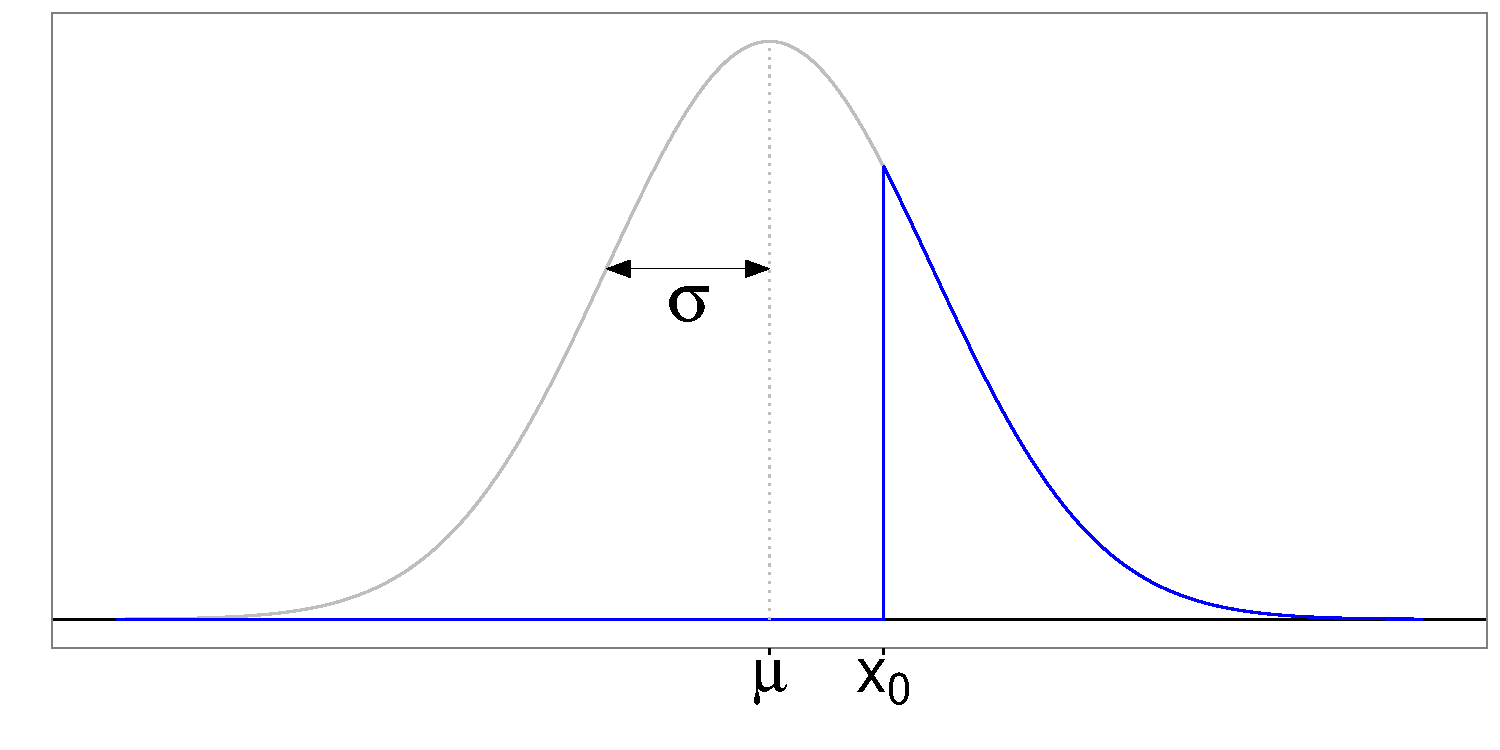
\includegraphics[scale=0.35]{figures/truncated-normal.pdf}
\caption{Truncated normal}
\label{trun-norm}
\end{figure}

The density $f$ has the following expression.
$$
f(x) = \frac{1}{(1 - \Phi(z_0))\sigma\sqrt{2\pi}}\;
\mathrm{e}^{-\frac{1}{2}\big(\frac{x-\mu}{\sigma}\big)^2}, \qquad x >
x_0
$$
where $\Phi$ is the cdf of the standard normal curve and $z_0 = (x_0-\mu)/\sigma$.

The cdf of $F$ has the following expression.
$$
F(x) =
\frac{\Phi\big(\frac{x-\mu}{\sigma}\big)-\Phi(z_0)}{1-\Phi(z_0)}
$$

Here is a derivation:
\begin{eqnarray*}
F(x) & = & 1 - \int_x^\infty \frac{1}{(1 - \Phi(z_0))\sigma\sqrt{2\pi}}\;
\mathrm{e}^{-\frac{1}{2}\big(\frac{t-\mu}{\sigma}\big)^2} \,\mathrm{d}t \\
& = & 1 - \frac{1}{1 - \Phi(z_0)}
\int_{\frac{x-\mu}{\sigma}}^\infty \frac{1}{\sqrt{2\pi}}
\mathrm{e}^{-\frac{z^2}{2}}\, \mathrm{d}z \\
& = & 1 - \frac{1 - \Phi(\frac{x-\mu}{\sigma})}{1 - \Phi(z_0)} \\
& = & \frac{\Phi\big(\frac{x-\mu}{\sigma}\big)-\Phi(z_0)}{1-\Phi(z_0)}, \qquad x > x_0
\end{eqnarray*}

Using the inverse cdf method, we can generate a random variable with distribution $F$
by the following equation where $U \sim \text{Uniform}(0,1)$.
$$
X = \mu + \sigma \Phi^{-1}( 1 - (1-U)(1-\Phi(z_0)))
$$
The derivation is straightforward.

Finally, whenever $z_0>7$, we use an exponential distribution, instead
of truncated normal because of numerical issues.

\subsection{Computation of the weights}
We computed the likelihood of the data given the drawn $\theta = (\mathbf{Q}, T,
\lambda)$ and evaluated the importance sampling density $g(\theta|X)$
to obtain the weight:
\begin{equation}
w(\theta) = \frac{L(\theta|X)}{g(\theta|X)}.
\end{equation}

Finally, we repeated the process to obtain an independent sample
$\theta_1, \theta_2,...,\theta_n \sim g(\theta|X)$ with the
unnormalized weights $w(\theta_1), w(\theta_2),...,w(\theta_n)$. Note
that since the likelihood used is not a normalized density, we are in
the case of self-normalizing importance sampling estimates, and thus,
we need to normalize the weights:
\begin{equation}
\tilde{w}(\theta_j) = \frac{w(\theta_j)}{\sum_{i=1}^n w(\theta_i)}.
\end{equation}

todo:
- add here the whole algorithm of bistro
- describe h functions of interest: indicator of tree


\section{Examples}
\label{examples}
here we present examples

\section{Discussion}
\label{discussion}
problems

- correlation of branch lengths: if all three branches are equal size,
then almost uncorrelated, but if one if long, the other two are correlated
- dimensionality: at the end we did not see this problem much
- clade distribution: if bistro mean and mb mean are far apart, our
clade distribution will not be good (use mds plots to show)
problems, limitations: two components: sample topolgy, and then
sample BL. the second one is good, but the other one: there are
cases when the shrinking of bootstrap towards the mean is good, in
other not 
- setting priors on pi,s, the dirichlet is fine, but in
the posterior is not really dirichlet (and we came up with the
generalized dirichlet

\backmatter

%%%%%% include this section if you wish to acknowledge people,
%%%%%% grant support, etc.

\section*{Acknowledgements}

The authors thank blabla.\vspace*{-8pt}

%%%%%% include this section only if your manuscript refers to supplementary
%%%%%% materials -- see Instructions for Authors at 
%%%%%% http://www.tibs.org/biometrics

\section*{Supplementary Materials}

Web Appendix 1 referenced in Section xxx is available
with this paper at the Biometrics website on Wiley Online Library.
\vspace*{-8pt}


\bibliographystyle{biom} \bibliography{bistro}

\appendix

\section{}
\subsection{Importance Sampling Background}
\label{background}
% Explain here what is importance sampling in general terms, explain
% normalized case and unnormalized case

Let $X \sim f(x)$, and suppose that we want to calculate the
expectation of a function $h(X)$ under $f(x)$:
\begin{equation}
E_f(h(X)) = \int h(x) f(x) dx := \mu
\end{equation}
If the integral does not have a closed solution, we can estimate $\mu$
with the mean from a random sample $X_1,X_2,...,X_n \sim f(x)$:
\begin{equation}
\hat{\mu} = \frac{1}{n} \sum_{i=1}^n h(X_i)
\end{equation}

\paragraph{Problem} It can be hard (or impossible) to get random samples
from $f(x)$.

\paragraph{Solution} Sample from an easier density $g(x)$ such that inference of $h(X)$ under $f(x)$ can be approached as
inference of $h(X)w(X)$ under $g(x)$ for a weight function
$w(x)=f(x)/g(x)$ defined when both $f(x)$ and $g(x)$ are \textit{normalized} densities (we will discuss the
    \textit{unnormalized} case in next subsection). That is,
\begin{eqnarray*}
E_f(h(X)) &= \int h(x) f(x) dx \\ 
&= \int h(x) \frac{f(x)}{g(x)} g(x) dx \\
&= \int h(x) w(x) g(x) dx \\
&= E_g(h(X)w(X))
\end{eqnarray*}

\paragraph{Importance Sampling Algorithm} The goal is to estimate
$\mu = E_f(h(X))$, and $\sigma^2 = Var_f(h(X))$.
\begin{enumerate}
\item{Sample independently $Y_1,Y_2,...,Y_m \sim g(x)$}
\item{Define the weight function: $w(x) = f(x)/g(x)$}
\item{Mean estimate: $\hat{\mu} = \frac{1}{m} \sum_{i=1}^m
    h(y_i)w(y_i)$}
\item{Variance estimate: $\hat{\sigma}^2 = \frac{1}{m} \sum_{i=1}^m
    (h(y_i)w(y_i) - \hat{\mu})^2$}
\end{enumerate}


\paragraph{Standard error}
Since $Y_1,Y_2,...,Y_m \sim g(x)$ is an independent sample, we can
compute the variance of the estimator as
\begin{equation}
Var_g(\hat{\mu}) = \frac{1}{m} Var_g(h(X)w(X)) = \frac{\sigma^2}{m}
\end{equation}

\subsubsection{Unnormalized case}
The usual approach of importance sampling assumes that you have the
normalized versions of both $f(x)$ and $g(x)$. In many real-life
applications, this is not true.

Let $X \sim f(x) = c_1 f_0(x)$, and we again want to estimate
$E_f(h(X))$. We sample independently $Y_1,Y_2,...,Y_m \sim g(x) = c_2
g_0(x)$.
Unlike in the previous setting, we compute the weights with the
\textit{unnormalized} densities: $w_0(y_i) = f_0(y_i) / g_0(y_i)$.

This unnormalized case is different from the normalized importance
sampling case. Here we do inference of $h(X)$ directly, but
with a weighted sample $Y_1,Y_2,...,Y_m$ with weights
$\tilde{w}_0(y_1),\tilde{w}_0(y_2),...,\tilde{w}_0(y_m)$ with
$\tilde{w}_0(y_j) = \frac{w_0(y_j)}{\sum_{i=1}^m w_0(y_i)}.$ On the
contrary, in the normalized importance sampling case, we do inference
of $h(X)w(X)$ with a random sample from $g(x)$.

\paragraph{Unnormalized Importance Sampling Algorithm} The goal is to estimate
$\mu = E_f(h(X))$, and $\sigma^2 = Var_f(h(X))$.
\begin{enumerate}
\item{Sample independently $Y_1,Y_2,...,Y_m \sim g(x)$}
\item{Define the weight function: $w_0(y_j) = f_0(y_j)/g_0(y_j)$, and
    the normalized weight as $\tilde{w}_0(y_j) =
    \frac{w_0(y_j)}{\sum_{i=1}^m w_0(y_i)}.$}
\item{Mean estimate: $\hat{\mu} = \sum_{i=1}^m
    h(y_i)\tilde{w}_0(y_i)$}
\item{Variance estimate: $\hat{\sigma}^2 = \sum_{i=1}^m
    (h(y_i) - \hat{\mu})^2 \tilde{w}_0(y_i)$}
\end{enumerate}

The estimate $\hat{\mu}$ is sometimes called
\textit{self-normalized importance sampling estimate}.

\paragraph{Standard error}
Since the sample $Y_1,Y_2,...,Y_m$ with weights
$\tilde{w}_0(y_1),\tilde{w}_0(y_2),...,\tilde{w}_0(y_m)$ is no longer
an independent sample (because weights add up to 1), the variance
estimate is then \citep{Owen2013}
\begin{equation}
\widehat{Var}(\hat{\mu}) = \sum_{i=1}^m \tilde{w}_0(y_i)^2(h(y_i)-\hat{\mu})^2.
\end{equation}

\subsubsection{Diagnostics}
Importance sampling diagnostics are not clear-cut rules. One common
approach is to compute the effective sample size:
\begin{equation}
n_e = \frac{\left( \sum_{i=1}^n w(y_i) \right)^2}{\sum_{i=1}^nw(y_i)^2}.
\end{equation}

If the effective sample size is too small, then one or few weights
could be too large compared to the others, and importance sampling is
not as efficient as expected.


\label{lastpage}

\end{document}

% - status quo is mcmc, successful but computationally inefficient
% (reference ronquist paper) 
% - use IS as alternative 
% - show methods
% - show examples (improvement in ESS does not translate to improvement
% in time, we do a lot more computation per tree) 
% - discussion: problems, limitations: two components: sample topolgy, and then
% sample BL. the second one is good, but the other one: there are
% cases when the shrinking of bootstrap towards the mean is good, in
% other not 
% - setting priors on pi,s, the dirichlet is fine, but in
% the posterior is not really dirichlet (and we came up with the
% generalized dirichlet, maybe a separate paper)
